\documentclass[twocolumn,11pt]{article}
\usepackage{amsmath}
\usepackage[margin=1in]{geometry}
\usepackage{graphicx}
\usepackage{import}
\usepackage{subfig}

\title{Vision-Based Autonomous Ground Vehicle Navigation}
\date{May 2, 2011}
\author{
	Michael Koval \\
	mkoval@eden.rutgers.edu \\
	Electrical and Computer Engineering
}

\begin{document}
\maketitle

\section{Introduction}
\label{sec:intro}
% 1. Overall description of IGVC
The Intelligent Ground Vehicle Competition (IGVC) is an international
collegiate robotics competition that tasks each team to design,
build, and program a fully autonomous mobile ground vehicle.  Each successful
entry must autonomously navigate through an outdoor obstacle course using only
the sensors and computing power on-board the robot. As per the offical rules,
the competition is split into three parts: (1) navigating through a narrow
obstacle course delimited by painted white lines, (2) traveling between global
positioning system (GPS) waypoints scattered throughout a large field, and
(3) responding to Joint Architecture for Unmanned Systems (JAUS) messages to
autonomous control the robot ~\cite{igvc11}.

% 2. Importance of Perception
For each of these tasks, the robot is provided with only the GPS coordinates of
a destination way point and has knowledge of the course's topology. Without a
priori knowledge of the course boundaries and obstacles, navigating to the
destination requires that the robot build a map of its environment in
real-time. Using this map, the robot can plan a path through the drivable
regions of the course towards the final destination, avoiding obstacles and
avoiding the course boundaries at all costs. While the accuracy requirements
for the  perception and localization algorithms used to build a global map map
are significantly higher than simpler techniques, navigating with no high-level
view of the environment is much less effective.

% 3. Overview
Adding obstacles to the robot's internal representation of the world is
accomplished by merging the output of a scanning laser range finder (LIDAR) and
a custom stereo camera. In addition to identifying road obstacles, a successful
entry must also employ monocular image processing techniques to identify the
painted white lines that mark the course boundaries. Before discussing specific
obstacle and line detection algorithms, Section ~\ref{sec:robot} provides a
brief introduction to the hardware and software powering the Rutgers Navigator,
Rutgers University's entry into the 2011 IGVC.  The remainder of this paper is
split into two major sections: stereo reconstruction (Section
~\ref{sec:stereo}) for obstacle detection and monocular image processing
(Section ~\ref{sec:line}) for detecting the course boundary lines (Section
Finally, Section ~\ref{sec:econ} discusses the global impact of robotics: how
robots can assist in the recovery from major environmental disasters, such as
the recent earthquake off the cost of Japan.

\section{Rutgers Navigator}
\label{sec:robot}
% 1. Brief discussion of mechanical design
Designed specifically for rugged outdoor use and modularity, the Rutgers
Navigator (Figure ~\ref{fig:robot-photo}) is constructed entirely out of 80/20
extrusion and custom-machined aluminum stock. This provides a strong,
light\footnote{Approximately 100 lb empty and 150 lb fully loaded.} frame that
is much easier to modify than a conventional welded steel frame. This chassis
is supported by three wheels: two powered front wheels that are mounted on a
wish bone suspension for improved stability and free-spinning rear caster
chosen specifically to reduce friction while turning.

\begin{figure}
	\center
	% TODO: Update Photo
	% TODO: sensor rendering
	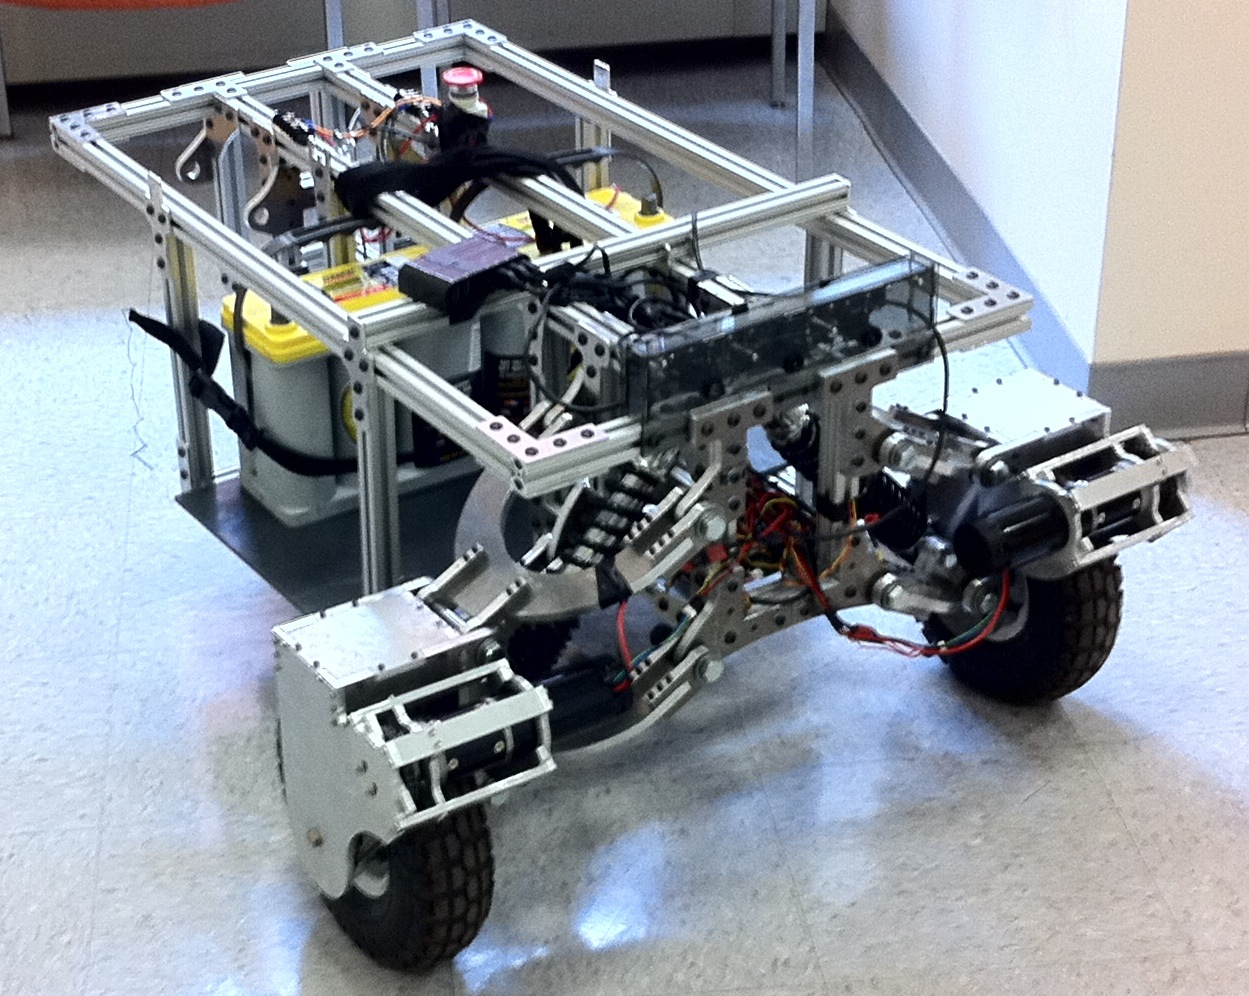
\includegraphics[width=\linewidth]{include/robot-photo}
	\caption{
		Rutgers Navigator. The front of the robot is equipped with three stereo
		stereo cameras on the front of the robot, and one camera located above
		each front wheel (not visible).
	}
	\label{fig:robot-photo}
\end{figure}

% 2. Sensing capabilities
\subsection{Sensing Capabilities}
\label{sec:robot-sensors}
Each of the four drive motors attached to the powered front wheels is equipped
with an internal hall-effect quadrature encoder to measure wheel speed and a
current sensor to monitor power consumption. The local odometry information
captured by the wheel encoders is combined with the data produced by a
nine-axis inertial measurement unit (IMU) to estimate the robot's motion.
Between the wheel encoders, accelerometer, gyroscope, and magnomiter, the
Navigator has access to a wealth of inertial data about its motion.
Unfortunately, all of these sensors share a common flaw: the tendancy to drift
over time by accumulating correlated error. Without frequent zeroing the
Navigator's position estimate to a known location, this type of localization
quickly becomes too inaccurate for long-term mapping.

To correct for the encoder and IMU drift, the Navigator uses a differential
global positioning system (DGPS) to measure its position in a globally fixed
coordinate frame. Using publically available differential correction signals
provided by the United States Coast Guard, the high-end Novatel DGPS on the
Navigator is capable of estimating the robot's position anywhere on the Earth
within 50 cm.  Combined with OmniStar's professional DGPS correction service,
the Novatel DGPS's accuracy increases to approximately 10 cm: a localization
error that is insignificant compared to the size of the robot. By fusing the
DGPS and the inertial position estimates with an enhanced Kalman filter, the
Navigator will both have an accurate estimate of its absolute position and its
relative motion over time.

As was discussed in Section ~\ref{sec:intro}, precise knowledge of the robot's
position is not sufficient to perform well in any of the IGVC challenges. To
detect obstacles in its environment, the Navigator uses the combination of a
high-end Hokuyo scanning laser rangefinder (LIDAR) and a custom trinocular
stereo camera that is discussed in detail in Section ~\ref{sec:stereo}.
Combining the high-resolution planar data returned by the Hokuyo LIDAR with the
stereo reconstruction of the scene, the navigator can take advantage of the
best features of both technologies: the Hokuyo's 270 degree horizontal field of
view and the stereo cameras' 75 degree vertical field of view. In addition to
the Hokuyo LIDAR and trinocular stereo camera, an additional angled camera is
mounted above each front wheel to identify painted boundary lines that cannot
be seen by the stereo cameras.

\subsection{Software Architecture}
\label{sec:robot-software}
Interaction between the robot's individual software components is managed
using the Robot Operating System (ROS), a framework developed by Willow Garage
to promote code reuse in robotics. Besides providing a common interface to
libraries such as OpenCV and PointCloud Library (PCL), ROS encourages the
separation of software into a graph of loosely-coupled \textit{nodes} that
communicate over TCP/IP sockets. Because each node \textit{subscribes} to its
inputs and \textit{publishes} its outputs with no global knowledge of the
system, it is possible to reuse nodes without ever modifying their internal
structure.

\begin{figure}
	\centering
	% TODO: update this image
	\includegraphics[width=\linewidth]{include/robot-software-vision}
	\caption{Computer vision software subsystem.}
	\label{fig:robot-vision}
\end{figure}

Figure ~\ref{fig:robot-vision} shows an overview of the flow of data between
nodes in the computer vision subsystem. Within this graph of nodes, there are
two distinct pipelines: stereo vision and monocular lane tracking. As its name
suggests, the \textit{stereo vision} pipeline (Section ~\ref{sec:stereo}) uses
triplets of synchronized images from the front stereo camera to generate a
three-dimensional point cloud of obstacles. The monocular \textit{line
tracking} (Section ~\ref{sec:line}) pipeline, conversely, processes images from
the left stereo camera and the two wheel cameras to find any white painted
lines that are in the Navigator's field of view. Detected lines are projected
into three-dimensional space and are directly added to the gobal navigation
grid as boundary obstacles.

\section{Stereo Vision}
\label{sec:stereo}
Unlike a laser rangerfinder, such as the Hokuyo UTM-30LN that was discussed in
Section ~\ref{sec:robot}, stereo vision is a passive sensor that reconstructs a
three-dimensional scene using two or more standard cameras placed at different
locations in space. By matching corresponding points between images captured by
the two cameras and using knowledge of their relative positions in space (i.e.
the \textit{baseline}), it is possible to completely reconstruct a three-dimensional
scene. While fairly straightforward with stationary cameras in a static scene,
using stereo vision on a moving platform poses many more problems.

Before discussing the actual scene reconstruction, Section
~\ref{sec:stereo-sync} discusses the process of \textit{hardware
synchronization} the Navigator's trinocular stereo camera. This guarantees that
the baseline remains constant even when the robot is driving at high speeds and
allows stereo vision to reliably work on a moving platform. Assuming that the
cameras are rigidly mounted and synchronized, Section ~\ref{sec:stereo-mux}
discusses the selection of a trinocular stereo system with a 10 cm
\textit{narrow} baseline and 20 cm \textit{wide} baseline the \textit{baseline
multiplexing} that fuses the data into a single reconstructed point cloud.
Using the combined point cloud, Section ~\ref{sec:stereo-algo} describes the
base stereo reconstruction algorithm used for triangulation and Section
~\ref{sec:stereo-od} details the post-processing processing steps needed to
identify obstacles in the reconstructed point cloud.

\begin{figure*}[t]
	\centering
	\subfloat[Unsynchronized \texttt{VSYNC}]{
		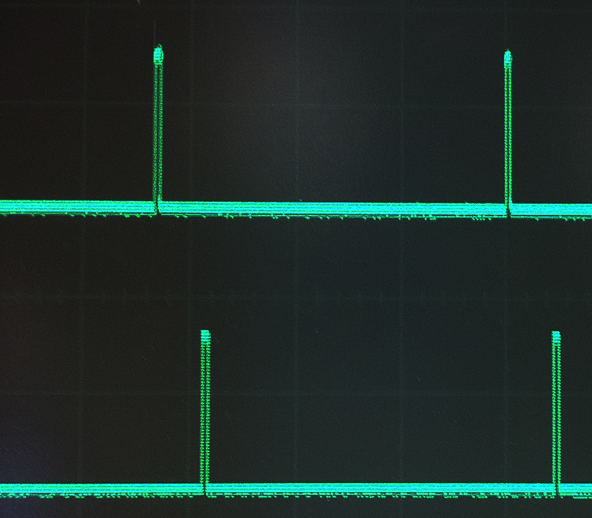
\includegraphics[width=0.24\textwidth]{include/unsync-scope}
		\label{fig:stereo-sync-hard1}
	}
	\subfloat[Synchronized \texttt{VSYNC}]{
		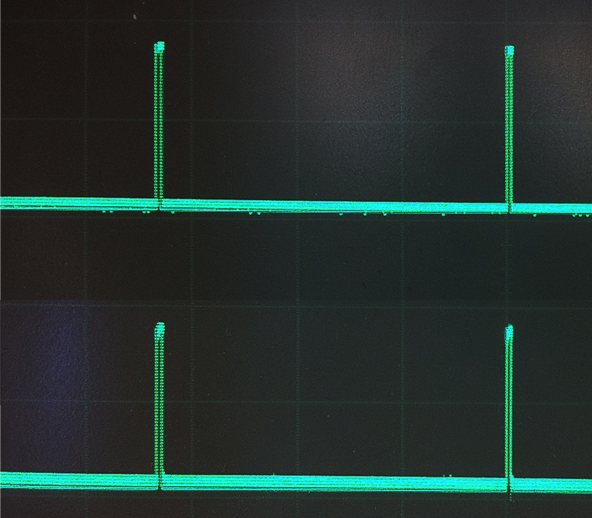
\includegraphics[width=0.24\textwidth]{include/sync-scope}
		\label{fig:stereo-sync-hard2}
	}
	\subfloat[Unsynchronized Frames]{
		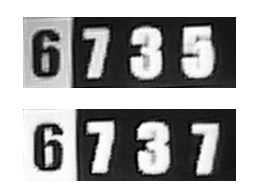
\includegraphics[width=0.24\textwidth]{include/unsync-img}
		\label{fig:stereo-sync-soft1}
	}
	\subfloat[Synchronized Frames]{
		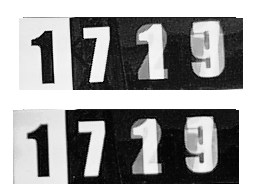
\includegraphics[width=0.24\textwidth]{include/sync-img}
		\label{fig:stereo-sync-soft2}
	}
	\caption{
		Verification of hardware and software camera synchronization for two
		Playstation Eye cameras. Note how only the synchronized cameras share a
		common \texttt{VSYNC} clock and capture identical readings of a
		millisecond resolution timer.
	}
	\label{fig:stereo-sync}
\end{figure*}

\subsection{Synchronization}
\label{sec:stereo-sync}
Stereo vision on a mobile robot is a non-trivial problem that has traditionally
expensive, hardware-synchronized machine-vision cameras. Because standard
stereo reconstruction assumes that the images from the left and right cameras
are captured from a common scene, any motion that occurs between the left and
right cameras capturing frames is equivalent to a change in the stereo camera's
baseline. This change in baseline invalidates the system's extrinsic
calibration\footnote{Capturing images at 30 Hz while moving at 10 mph could
change the baseline by up to 7 cm.}, causing the quality of the rectification
to decrease and the distances to be distorted by the robot's velocity
~\cite{unsync}.

Hardware synchronization, the process of forcing two or more cameras to share a
common hardware clock, has been traditionally limited to to professional stereo
visio systems such as Point Grey's Bumblebee product line.  Thankfully, the
inexpensive Playstation Eye camera is built on the same high-end OmniVision
OV7720 chipset that is comparable to those found in many machine vision
cameras. These cameras can be hardware-synchronized using the exposed frame
clock input (\texttt{FSIN}) and output (\texttt{VSYNC}) pins
~\cite{omnivision}. By shorting one camera's \texttt{VSYNC} pin to the other
cameras' \texttt{FSIN} pins, the cameras are forced to share a common clock. To
reduce the risk of a difference in ground potentials damaging the OV7720's
delicate circuitry, each camera was also modified to share a common ground.

This hardware synchronization guarantees that all three cameras capture images
simultaneously, but does not guarantee that the frames will remain synchronized
after USB transfer to the computer. Making direct use of the Video4Linux
kernel module, reliable synchronization was achieved by enabling memory-mapped
I/O for image transfering and fuzzy-matching the Linux kernel's USB transfer
timestamps\footnote{\texttt{https://github.com/mkoval/stereo\_webcam}}. Because
this matching algorithm uses the Linux kernel's USB transfer timestamps instead
of those measured in user-space, this simple algorithm is extremely robust to
periodic desynchronizations caused by dropped frames and increased USB latency.

Hardware synchronization was verified by probing each camera's \texttt{VSYNC}
pin with an oscilloscope (Figures ~\ref{fig:stereo-sync-hard1} and
~\ref{fig:stereo-sync-hard2}) and confirming that all three clocks are in
phase. The software synchronization was further verified by simultaneously
capturing images of a millisecond resolution timer (Figures
~\ref{fig:stereo-sync-soft1} and ~\ref{fig:stereo-sync-soft2} on all three
synchronized cameras. Since the times exactly match after synchronization and
differ by several milliseconds on the original unsynchronized cameras, the
camera synchronization is clearly a success. These three hardware-synchronized
Playstation Eye cameras are mounted in a custom polycarbinate case on the front
of the Navigator and serve as a custom trinocular stereo camera.

\subsection{Baseline Selection}
\label{sec:stereo-mux}
Selecting the optimal baseline for a stereo system is a balance of two
opposing, but equally important, factors: field of view and maximum range.
Decreasing the baseline increases the shared field of view of the two cameras
at the cost of a shorter maximum range. Conversely, increasing the baseline
decreases the aggregate field of view, but yields an increased maximum range
and better precision at each visible distance. Using a trinocular stereo system
instead of a standard binocular system allows the software to get the
advantages of two baselines with the addition of only one camera.

The \textit{narrow} pair has a baseline of approximately 10 cm and uses the
left and middle cameras. Conversely, the \textit{wide} pair has a baseline of
approximately 20 cm and uses the left and right cameras. By using the narrow
baselines for nearby points and the wide baseline for more distance points,
this trinocular stereo system combines the small minimum range of the narrow
baseline with the better accuracy and maximum range of the wide baseline.

\begin{figure*}
	\centering
	\subfloat[Multiplexed Point Cloud]{
		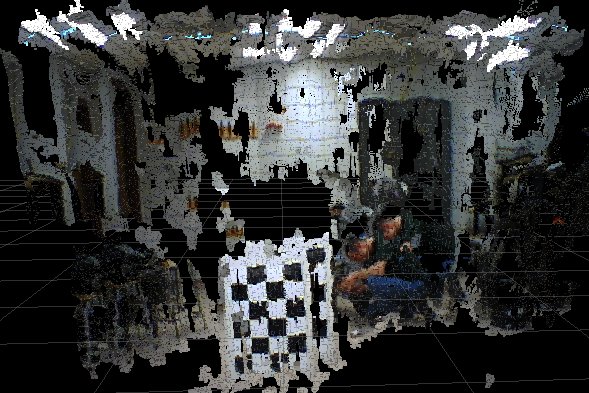
\includegraphics[width=0.5\linewidth]{include/stereo-both}
	}
	\subfloat[Reconstruction Error]{
		\subimport{include/}{stereo-dist}
	}
	\caption{
		Reconstructed point cloud using stereo multiplexing. Differences in the
		camera's rectification and reconstruction accuracy cause a small
		rotation in the reconstructed point cloud.
	}
	\label{fig:stereo-dist}
\end{figure*}

\subsection{Reconstruction Algorithm}
\label{sec:stereo-algo}
Due to the use of ROS as the basis for the Navigator's software architecture
(Section ~\ref{sec:robot}), the actual stereo reconstruction is done using the
standard \texttt{stereo\_image\_proc} ROS node. Before being processed for
point correspondences, the pair of input images is rectified, regions of low
texture are masked out, and a Sobel filter is applied to amplify texture
~\cite{stereo}. Each pixel in the left image is matched to the most similar
pixel in the corresponding row in the right image using a sum-of-squared
difference (SSD) block-matching algorithm ~\cite{stereo} and the corresponding
disparity is calculated.  This disparity is then converted to a
three-dimensional point using the camera's intrinsic parameters.

While more efficient than the graph-cut based alternatives, ~\cite{stereo} the
SSD block-matching algorithm implemented in the ROS
\texttt{stereo\_image\_proc} is still extremely computationally intensive. With
all three cameras set to a resolution of $640 \times 480$ and a frame rate of
15 Hz, the stereo block-matching algorithm runs at approximately 10-12 Hz.
While this is much slower than the 60 Hz maximum frame rate of the cameras, it
is more than sufficient considering the rate at which the path planning
algorithm executes.

\subsubsection{Ground Plane Detection}
\label{sec:stereo-ground}
When travelling over uneven terrain such as grass, the position and orientation
of the cameras can change relative to the ground as the robot moves. Compounded
by perspective projection, the effect of this movement is very detrimental to
algorithms that rely on knowledge of the ground plane such as stereo obstacle
detection (Section ~\ref{sec:stereo-od}) and the matched pulse-width filter
used for line detection (Section ~\ref{sec:line}). Analysis of recorded video
that has been processed by the above reconstruction algorithm shows that the
block-matching algorithm described in Section ~\ref{sec:stereo-algo} detects
sufficient texture on the ground to produce a dense disparity map.

Assuming that the ground is a perfect plane parameterized by $a$, $b$, $c$, and
$d$, a large number of reconstructed points are described by the model
\begin{equation}
	ax + by + cz + d = 0,
	\label{eq:stereo-ground}
\end{equation}
where $(x, y, z)$ are the reconstruction points position in three-dimensional
space.

Once stereo vision has reconstructed the three-dimensional scene in front of the
Navigator, the Random Sample and Consensus (RANSAC) model-fitting algorithm is
used to fit Equation ~\ref{eq:stereo-ground} to the ground plane. Unlike least-squares estimation and other primitive
model-fitting algorithms, RANSAC is a robust iterative algorithm that
\textit{randomly samples} the data to find a model that has minimizes minimizes
the model error for some \textit{concensus set} of inliers. Assuming that the
ground plane is the dominant plane in the image and that RANSAC is run for a
suficient number of iterations, RANSAC classifies points on the ground plane as
inliers and all other points, such as obstacles, as outliers.

Unfortunately, the assumption that the ground plane will dominant other planes
in the image is only accurate if the region in front of the robot is relatively
empty. When the robot is facing a nearby obstacle, RANSAC may inappropriately
fit a plane to obstacle points instead of the non-existant ground points. Since
such a situation would rotate the ground plane by approximately 90 degrees, a
manually-tuned decision tree is used to reject poor fits. This decision tree
eliminates models that have too few inliers, are at too high of an angle, or
hae too large a vertical offset from the robot. Simulation and experimental
testing using a heavily textured plane show that this decision tree eliminates
the vast majority of false ground plane detections.

\subsubsection{Obstacle Detection}
\label{sec:stereo-od}
Once the ground plane has been found and the inlier points have been removed,
the remainder of the point cloud is assumed to be a mix of obstacle points
and outliers caused by incorrect point correspondances. As the Navigator uses
a path planner that does not explicitely deal with uncertaintanty, these false
positives must be removed before detected obstacles are added to the map used
for path planning.

Assuming that correctly detected obstacles dominate the remaining points, the
obstacle detection problem is reduced to an outlier detection on a
three-dimensional point cloud. Properly reconstructed points that belong to an
object are likely to form large clusters and outliers are likely to remain
fairly isolated. If an obstacle point is selected at random, one would expect
that the standard deviation of the $x$, $y$, and $z$ coordinates of its $k$
nearest neighbors to be relatively low. For an isolated outlier, the same
calculation would produce an abnormally high stadard deviation
~\cite{rusu2008towards}. By repeating this process on every point and
classifying all points with a sufficiently high standard deviation as outliers,
spurious detections from poor point correspondances are completely eliminated
~\cite{rusu2008towards}. Once outliers have been removed, the resultant point
cloud can safely be added to the robot's internal map.

\subsection{Error Analysis}
\label{sec:stereo-error}
After the stereo cameras were calibrated using a modified version of the ROS
camera calibration toolkit, the depths reported by both stereo baselines were
measured and compared to ground truth. Measuring the ground truth data from 0
to 8 meters (Figure ~\ref{fig:stereo-dist}), the narrow stereo pair's dead
zone of 0.9 meters is approximately half the size of the wide stereo pair's
dead zone of 1.6 m. As distance increases beyond 3 m, the wide baseline begins
to surpass the narrow baseline in accuracy. In additition to manual measurements
with a calibration chessboard, these results were confirmed by using the Hokoyu
LIDAR for ground-truth distances. Even when objects are several meters away,
the depths calculated by the stereo vision system match those measured by
the Hokuyo LIDAR within several inches.

\section{Lane Tracking}
\label{sec:line}
For both the navigation and GPS challenges, the drivable region of the course
is delimited by a three inch wide line painted on grass or asphalt.
Robustly identifying and tracking these boundary lines is a
difficult problem that has been the primary cause of disqualification in
previous years of competitions. For example, 28 out of 29 competitors were
disqualified failing to move, leaving the course, or striking an obstacle
before five minutes time limit elapsed in the 2010 IGVC.

To avoid repeating the errors made by teams in previous years, the Navigator
simultaneously runs an advanced line detection algorithm on images from three
cameras: the center stereo camera, the left wheel camera, and the right wheel
camera. The front-facing stereo camera provides the long-term knowledge of the
course shape necessary for path planning, while the left and right insure that
the Navigator does not inadvertantly cross a line while following a long-term
path. By fusing the line detetion results from all three cameras, the
Navigator's field of view is expanded from 75 degrees to nearly a full 180
degrees.

The line detection algorithm run in parallel on each camera is a modified
version of the algorithm used by Massachusetts Institute of Technology's entry
into the DARPA Grand Challenge.  In this algorithm, a color image of the course
first undergoes a color space transformation to emphasize white regions of the
image (Section ~\ref{sec:line-color}). The grayscale output of the color space
transformation is then filtered using a matched pulse-width filter (Section
~\ref{sec:line-filter}) that eliminates lines of the incorrect width. Finally,
the size of the output point cloud is compressed using non-maximal suppression
(Section ~\ref{sec:line-max}) and the detected local maxima are transformed
into the world coordinate frame to be directly used for navigation
~\cite{huang_thesis} ~\cite{huang_paper}.

\begin{figure*}[t]
	\centering
	\subfloat[Original Image]{
		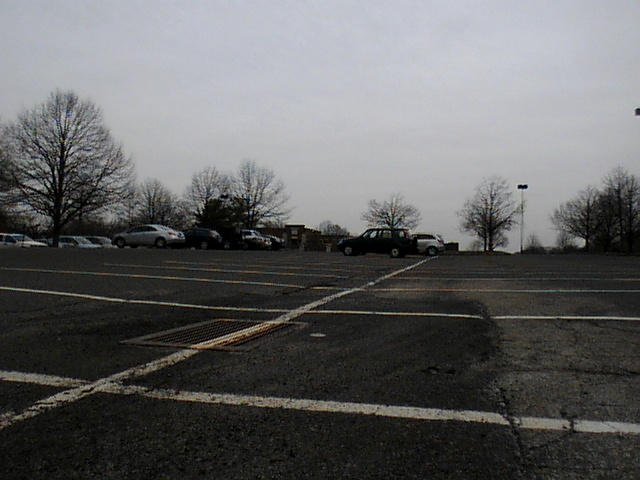
\includegraphics[width=0.45\linewidth]{include/line-orig}
	}
	\subfloat[Color Space Transformation]{
		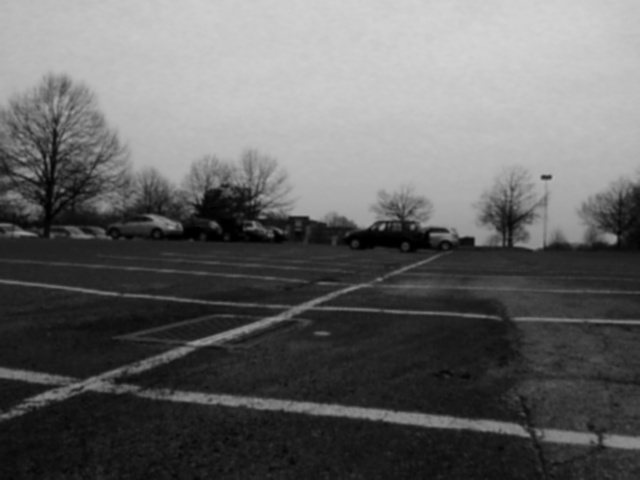
\includegraphics[width=0.45\linewidth]{include/line-pre}
	}
	\\
	\subfloat[Matched Pulse-Width Filter]{
		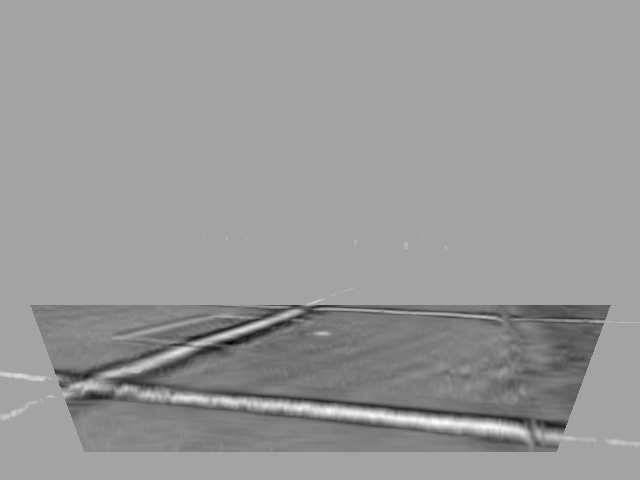
\includegraphics[width=0.45\linewidth]{include/line-filter}
	}
	\subfloat[Non-Maximal Suppression]{
		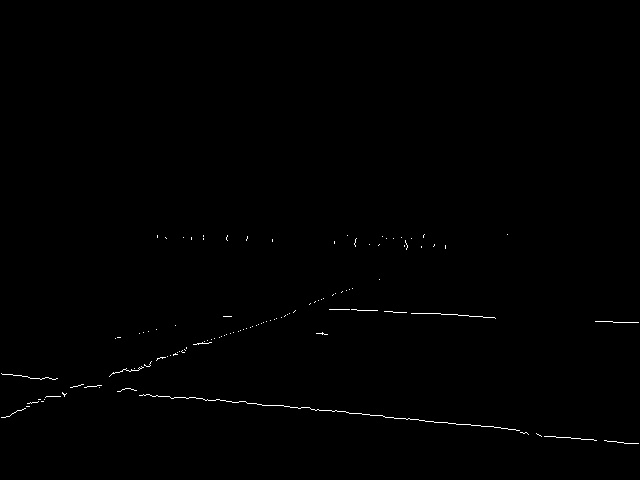
\includegraphics[width=0.45\linewidth]{include/line-max}
	}
	\caption{
		Intermediate stages of the line detection algorithm. Each stage of
		processing removes filters unnecessary data from the image and
		simplifies the remainder of the processing pipeline.
	}
	\label{fig:line-all}
\end{figure*}

\subsection{Extrinsic Calibration}
\label{sec:line-extrinsic}
While the addition of two wheel cameras greatly expands the Navigator's field
of view, the images are only useful if they are captured in a known coordinate
frame. As the stereo camera is calibrated against the LIDAR, the extrinsic
calibration of the wheel cameras can be simplified to finding their pose
relative to the stereo camera. Using a process common in calibration, a small
chessboard is placed in the shared field of view of the two cameras. Each of
the detected grid corners, $p_1, p_2, \cdots, p_n$ are assigned three-dimensional
coordinates in a coordinate frame aligned with the chessboard: $P_1, P_2, \cdots
P_n$.

Using the camera's intrinsic matrix and the definition of perspective projection,
the relationship
\begin{equation*}
	\tilde{p}_i = M_{int} T \tilde{P}_i
\end{equation*}
must hold for each point, where $T$ is the transformation from the chessboard
frame to the camera frame. Expanding the matrix multiplication $T P_i$, this
can be rewritten as $M_{int}^{-1} \tilde{p}_i = T \tilde{P}_i$ and $T$ is found
using least-squares estimation.

To calibrate one camera relative to second camera, this calibration procedure is
repeated on a pair of synchronized frames. Since the same chessboard is seen in both views,
$T_1$ is the transformation from the chessboard to camera 1 and $T_2$ is the
transformation from the same chessboard to camera 2. Both transformations are
expressed in a common coordinate frame and the transformation from camera 2 to camera
1 is simply $T_{12} = T_1 T_2^{-1}$. Using this calibration technique to solve for
the position of the left and right wheel cameras relative to the center stereo camera
makes it possible to accurately transform coordinates generated in all three cameras
into a common coordinate frame that can be used for navigation.

\subsection{Color Space Transformation}
\label{sec:line-color}
Using a priori knowledge that the lines are white, the first step towards
effectively isolating them from their surroundings is to convert the rectified
color image into a monochromatic color space where white is amplified. Because
white is inherently of high intensity and low saturation, the
hue-saturation-value (HSV) color space is a natural choice. If the original
image, $I_{orig}$, has the 8-bit HSV channels $H(x,y)$, $S(x, y)$, and $V(x,
y)$, define the pre-processed image $I_{pre}$ to be
\begin{equation*}
	I_{pre}(x, y) = \min\left\{255 - S(x, y), V(x, y)\right\}
\end{equation*}
for each pixel $(x, y)$ in $I_{orig}$.

\subsection{Matched Pulse-Width Filter}
\label{sec:line-filter}
In addition to the lines' color, the 2011 IGVC rules specify that all painted
lines will be uniformly three inches wide. Using this knowledge of the line's
width, an  obvious approach for isolating them from other objects is to use a
digital \textit{pulse-width filter} that responds strongly to objects with the
same width as a line. Unfortunately, effect of perspective projection causes
the apparent width of lines in an image depend upon their distance from the
camera and position in three-dimensional space. To obtain meaningful output,
such a filter must be properly \textit{matched} to expected width of the line
for each point in the input image ~\cite{huang_thesis} ~\cite{huang_paper}.

Calculating this width requires knowledge of the three-dimensional point
corresponding to each pixel in the image. Assuming that the ground plane is
known and is parametrized by point $P$ and normal $n$, the three-dimensional
point $P$ that corresponds to pixel $p$ satisfies both
\begin{align*}
	(P - P_0) \cdot n                  &= 0 \\
	\lambda M^{-1}_{int} p - \tilde{P} &= 0,
\end{align*}
where $M_{int}$ is the camera's intrinsic matrix and $\lambda$ is an arbitrary
constant.

Solving for $\lambda$ gives a closed-form expression expressed in terms of only
known parameters Substituting this definition of $\lambda$e into the equation
of the line yields an intersection point of
\begin{equation*}
 	P = \left(\frac{n \cdot \tilde{P}_0}{n \cdot M^{-1}_{int} p}\right) M^{-1}_{int} p.
	\label{eqn:line-point}
\end{equation*}
Using the new-found knowledge of point $P$, the length of an arbitrary real-world
vector projected into the image at point $p$ is
\begin{equation}
	\delta = ||M_{int} \tilde{P} - M_{int} (\tilde{P} + \Delta)||_2
	\label{eqn:line-width}
\end{equation}
where $\delta$ is the image distance corresponding to a change in world
coordinates by the vector $\Delta$ and $||\cdot||_2$ denotes the Euclidean
norm. Note that this is not equivalent to $||M_{int}\Delta||_2$ because of the
division implicit in the use of homogeneous coordinates.

Using this equation, the four distances of interest depicted in Figure
~\ref{fig:line-sketch} are projected into the image using Equation
~\ref{eqn:line-width}. Of these four distances, $\delta_{LL}$ and $\delta_{LR}$
correspond to the left and right edges of the line, respectively. Similarly,
$\delta_{BL}$ and $\delta_{BR}$ correspond to the expected total width of the
filter (including a dead zone around the line). Note that the filter is only
symmetric (i.e. $\delta_{LL} = \delta{LR}$ and $\delta_{BL} = \delta_{BR}$) for
the horizontal filter kernel. The vertical filter is asymmetric and shifted due
to perspective projection disproportionately elongating distances that are closer
to the camera.

Once the four widths have been projected into the image, a filter kernel is
constructed such that each of the negative \textit{supports} sums to $-0.5$
and the central \textit{pulse} sums to $+1.0$. This causes the filter to have
a zero response on solid color and to only respond strongly to lines of the
correct width and orientation. The region surrounding each pixel in the image
is convolved with both the horizontal and vertical matched filters and the
responses are ready for post-processing.

\subsection{Non-Maximal Suppression}
\label{sec:line-max}
The matched pulse-width filter is extremely effective at isolating the line in
the image, but does not produce a clean enough output to be directly used for
model-fitting. In particular, the nature of digital filters guarantees that
there will be weak, spurious responses near true positives.

Inspired by Canny edge detection, non-maximal suppression is an effective and
computationally efficient way of reducing such a response to a single point.
Considering the rows of the horizontally filtered image and the columns of the
vertically filtered image, a pixel is considered a maximum if and only if it
has a higher filter response than both of its neighbors. The maxima are then
thresholded to discard those that do not exhibit a sufficiently strong filter
response. This threshold was tuned to favor false positives and was set to
approximately 15\% of the filter's maximum response.

\begin{figure}
	\centering
	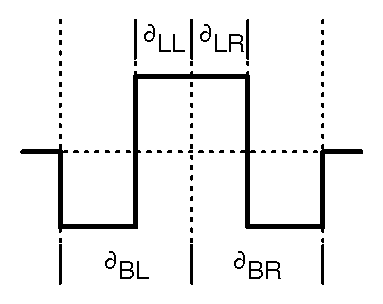
\includegraphics[width=0.6\linewidth]{include/line-sketch}
	\caption{Sketch of the matched pulse-width filter's kernel.}
	\label{fig:line-sketch}
\end{figure}

\subsection{Error Analysis}
\label{sec:line-error}

Largely because this algorithm is rooted in physical constants, and has few
arbitrary thresholds, this line detection algorithm works equally well in
simulation and on real data. 

Constructing the matched pulse-width filters succeeds even with large
variations in the ground plane, but those filters no longer match the width of
the line in the image.  Even worse, the detected line points in the world
appear at the wrong distance from the image. Tested on both simulated data and
real data, the algorithm appears very effective at identifying lines even in
noisy environments (e.g. the parking lot in Figure ~\ref{fig:line-all}).

\section{Conclusion}
\label{sec:conclusion}
After extensive testing of the custom stereo camera using an oscilloscope, a
millisecond resolution timer, and outdoor data, it is clear that the three
cameras are well synchronized. This synchronization translates into an
extremely high quality reconstruction while the robot is moving, giving it the
rich three-dimensional information required for path planning. Applying a
matched pulse-width filter to detect the lines bordering the field successfully
corrects for the effects of perspective transform and reliably detects both
horizontal and vertical lines in the image.

\section{Current Trends in Robotics}
\label{sec:econ}
% 1. Search and Rescue
The recent Japanese earthquake and tsunami was one of the worlds' most
devastating natural disasters. While the Japanese people's efficient response
captivated international news, it rapidly became clear manual search and rescue
is not feasible on a large scale. Every volunteer slowly climbs through debris
of collapsed buildings, moving a few miles per hour and putting his or her own
life at risk. This means that rescue volunteers are restricted to areas that
have been deemed sufficiently safe to walk: potentially denying access to some
of the surviors who are in most urgent need of assistance.

One solution to the search and rescue problem is to deploy teleoperated
tank-like robots to search debris for survivors ~\cite{search}. While still
controlled by a human, these search and rescue robots are equipped with
infrared cameras and carbon dioxide sensors to detect the presence of humans
that would otherwise go unnoticed ~\cite{search}. Even better,
this type of robot completely eliminates the need for rescue workers to enter
dangerous areas: it can be remotely deployed and controled from a safe
distance without putting any emergency workers to risk. While these robots are
not revolutionary, they do have a past history of success for mine rescues
~\cite{mine} and on September 11th ~\cite{sept11}.

While these robots remove human rescue workers from harms way, each robot is
too costly to be deployed in bulk. Replacing one large robot with a large
number of inexpensive, ``disposable'', robots is a better solution for
exploring dangerous environments such as collapsed buildings. One research
group at the University of California at Berkeley has developed just that: an
extremely inexpensive ``mechanical cockroach'' that is capable of fitting
through small cracks in rubble ~\cite{cockroach}. Based on the principles of
swarm robotics, using a large number of simple robots can give a cheaper and
more robust system than a small number of expensive robots. This is especially
the case in search and rescue: covering a wide area and being robust to extreme
environmental conditions is much more important than access to expensive,
high-accuracy sensing equipment. Even if a number of the robots are destroyed,
the remaining robots are completely independent and can continue to aid the
rescue effort.

For either of these techniques to become practical, the next major efficiency
improvement will be from replacing the human teleoperator with a fully
autonomous control system. This is especially important when using swarm
robotic rescue system: while it may be feasible to have a dedicate teleoperator
for a few smaller robots, it is completely infeasible for a large-scale swarm
system. Once the necessary advances have been made in producing inexpensive
mobile robots, a completely autonomous swarm robotics rescue system will be the
ideal solution for search and rescue: it is inexpensive, requires little
supervision, and allows humans to focus on tasks that are not as easy to
automate.

% 2. Infastructure Evaluation and Repair
Search and rescue is only the first step in disaster recovery. Once the
immediate disaster response is complete, the affected governments must begin
the long and arduous process of repairing and replacing their damaged
infastructure. With the extent of damaged caused by a natural disaster on the
scale of the Japanese earthquake, it is not safe to open roads, bridges, or
tunnels until they have been fully inspected and deemed structurally stable.
This, unfortunately, means that engineers must enter the compromised (and
potentially dangerous) structure to search for damage. Just like search and
rescue, this is a natural task for a teleoperated robot.

Instead of the engineers directly inspecting the damage, a robot can be
remotely controlled from a safe distance away from the damaged structure. Even
better, the inspection robot can carry sensors that a human cannot. These might
include a high-resolution camera ~\cite{gym} for inspecting damage to beams, a
scanning laser rangefinder for building a three-dimensional model of the
damage, or even a sensor package for measuring the concentration of airborn
contaminents. This type of remote inspection is crucial for disasters such as
the Deepwater Horizon, where manual inspection of the disaster site would be
completely impossible.

% Conclusion
With robots just beginning to replace humans in dangerous and high-risk
enironments, the potential for future improvement is clearly visible. Using
teleoperated robots keeps the human operators out of harms way and gives them
access to task-specific sensors and equipment that would otherwise be
unavailable. Without worrying about his or her personal safety, the operator is
able to devote his or her full attention to the mission and focus on making the
rescue effort continue as smoothly as possible. In the future, a human operator
may not be needed at all: full autonomy will automate the monotonous drudgery
of disaster recovery and let humans focus on the tasks that are most important.

\section{Acknowledgments}
This project would not have been possible without the support of Dr. Predrag
Spasojevic as our faculty adviser or the help of the members of Rutgers IEEE
Student Branch. I am particularly grateful for Adam Stambler's excellent
leadership, Peter Vasilnak's mechanical design, and the faculty support of Dr.
Kristin Dana, Joe Lippencott, Steve Orbine, John Scafidi, and Dr. Stuart
Shalat. I would also like to thank our sponsors for their generous
contributions: Rutgers Engineering Governing Council, Knotts Corporation, 80/20
Inc., Optima Batteries, Github, IEEE Region 1, Novatel, and Omnistar.

{\footnotesize
\bibliography{interim}{}
\bibliographystyle{plain}
}
\end{document}
